\documentclass[11pt]{exam}
\usepackage{commonheader}
\usepackage{graphicx}
\graphicspath{ {./images/} }

% Use the following to toggle solutions/metas
 \printsolutions % uncomment me
 %\printmeta %

\discnumber{BONUS}
\title{Mock Midterm 2}
\date{March 12th, 2023}

\begin{document}
\maketitle

%%%%%%%%%%%%%%%%%%%%
% Asymptotics % NO VIDEO
%%%%%%%%%%%%%%%%%%%%

\section{Runtime Funtime}

\begin{questions}
\subimport{topics/asymptotics/easy/}{intnode.tex}
\subimport{topics/asymptotics/MockMidterm/}{Q3.tex}
\subimport{topics/asymptotics/medium/}{log-loop.tex}

\end{questions}


\\
\\
\\
\\
\\
\clearpage

%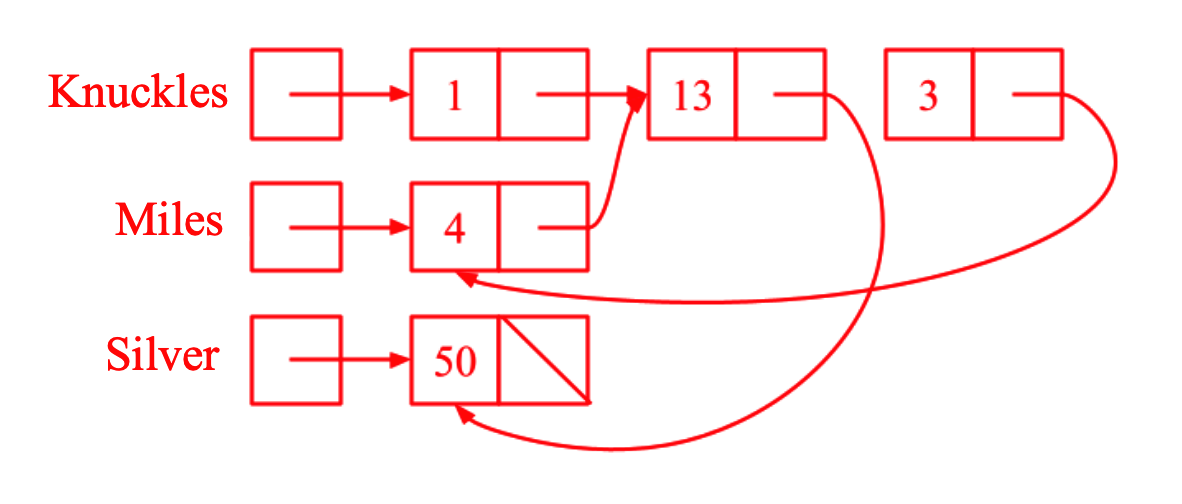
\includegraphics[scale=0.75]{sonic-box-pointers2.png}

\clearpage

%%%%%%%%%%%%%%%%%%%%
% BSTs % NO VIDEO
%%%%%%%%%%%%%%%%%%%%

\section{Height Matters?}

\begin{questions}
\subimport{topics/trees/binary-search-trees/easy/}{bst-valid-balanced.tex} 
\end{questions}

\clearpage


%%%%%%%%%%%%%%%%%%%%
% Hashing % NO VIDEO
%%%%%%%%%%%%%%%%%%%%

\section{Hashing Potpurri}

\begin{questions}
\subimport{topics/hashing/MockMidterm/}{Q1.tex}
\clearpage
\subimport{topics/hashing/MockMidterm/}{Q2.tex}
\end{questions}

\clearpage


%%%%%%%%%%%%%%%%%%%%
% Heaps
%%%%%%%%%%%%%%%%%%%%

\section{Heap Heap Hooray}

\begin{questions}
\subimport{topics/heaps}{example-tree.tex}
\subimport{topics/heaps/easy}{min-heapify.tex}
\end{questions}

\clearpage

%%%%%%%%%%%%%%%%%%%%
% Graphs
%%%%%%%%%%%%%%%%%%%%

\section{Munchlax Needs His Poffins}

\begin{questions}
%\subimport{topics/graphs/traversal}{implement-dfs.tex} CAN'T BE USED
\subimport{topics/graphs/traversal}{munchlax.tex}
\end{questions}

\clearpage

%%%%%%%%%%%%%%%%%%%%
% Asymptotic bounds of disjoint set problems 
%%%%%%%%%%%%%%%%%%%%

\section{Disjoint Sets}

\begin{questions}
\subimport{topics/union-find/weighted-quick-union/easy}{is-possible-short.tex}
\subimport{topics/union-find/weighted-quick-union/easy}{path-compression-find.tex}
\end{questions}


\end{document}
